\documentclass[12pt, letterpaper]{paper}
\usepackage{graphicx}
\usepackage{amsmath}
\usepackage{float}
 
\title{ Operations Research HW1 }
\author{ Timothy Schwieg }
\date { September 1st 2017 }

\begin{document}

\maketitle

\section*{Question 1}
Let x be the time in hours spent running process 1
\newline
Let y be the time in hours spent running process 2
\begin{equation*}
\begin{alignedat}{3}
&\text{min }&4x + y&\\
&\text{s.t. } &3x + y &\geq 10 \\
&  &x + y &\geq 5 \\
& &x &\geq 3\\
& & x &\geq 0\\
& &y &\geq 0
\end{alignedat}
\end{equation*}

\section*{Question 2}
Let x be the amount of books produced
\newline
Let y be the amount of couches produced
\newline
Let z be the amount of work tables produced
\begin{equation*}
\begin{alignedat}{3}
&\text{max }&6x + 5y + 8z&\\
&\text{s.t. } &12x + 14y + 16z&\leq 400 \\
&  &40x + 22y + 60z&\leq 1000 \\
& &x &\geq 0\\
& & y &\geq 0\\
& &z &\geq 0
\end{alignedat}
\end{equation*}


\section*{Question 3}
\begin{figure}[H]
\centering
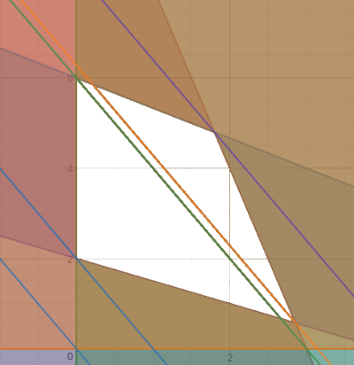
\includegraphics[width=0.8\textwidth]{q3.png}
\caption{ Feasible Set - Painted White }
\end{figure}
Since it is known that the maximum of a linear program will occur at an extreme point of the feasible set, we must only examine those points.
The points are $(0,2), (0,6), (\frac{20}{7},\frac{4}{7}), \text{and} (\frac{9}{5}, \frac{24}{5} )$ Evaluating f at each of these points we arrive at:
$f(0,2) = 2, f(0,6) = 6, f(\frac{20}{7},\frac{4}{7}) = \frac{44}{7} , f(\frac{9}{5}, \frac{24}{5} ) = \frac{42}{5}$ Thus the maximum is: $\frac{42}{5}$ occuring at: $(\frac{9}{5}, \frac{24}{5} )$ 



\section*{Question 4}
\subsection* {Part a. }

Consider the addition of $s_1, s_2, s_3$	
\begin{equation*}
\begin{alignedat}{3}
&\text{max }&2x + y&\\
&\text{s.t. } &4x + y + s_1&= 12 \\
&  &42x + 3y + s_2& = 18 \\
& &x + 2y - s_3 &= 	4\\
& & x &\geq 0\\
& & y &\geq 0\\
& & s_1 &\geq 0\\
& & s_2 &\geq 0\\
& & s_3 &\geq 0\\
\end{alignedat}
\end{equation*}

\subsection*{Part b.}
Since only the objective function has been changed, the feasible set remains unchanged, and the extreme points, where the maximum will occur, are unchanged. Thus the maximum must occur at $(0,2), (0,6), (\frac{20}{7},\frac{4}{7}), \text{or} (\frac{9}{5}, \frac{24}{5} )$
Evaluating f at each of these points we arrive at:
$f(0,2) = \frac{2}{5}, f(0,6) = \frac{6}{5}, f(\frac{20}{7},\frac{4}{7}) = \frac{304}{35} , f(\frac{9}{5}, \frac{24}{5} ) = \frac{104}{25}$ Thus the maximum is: $\frac{304}{35}$ occuring at: $(\frac{20}{7},\frac{4}{7} )$

\subsection*{Part c.}
Following the same procedure as Question 3, but minimizing the function instead.
$f(0,2) = 2, f(0,6) = 6, f(\frac{20}{7},\frac{4}{7}) = \frac{44}{7} , f(\frac{9}{5}, \frac{24}{5} ) = \frac{42}{5}$ Thus the minimum is: 2 occuring at: $(0,2)$

\section*{Question 5}

\subsection*{Part a.}
Let x be the number of desks made
\newline
Let y be the number of chairs made


\begin{equation*}
\begin{alignedat}{3}
&\text{max }&40x + 25y&\\
&\text{s.t. } &4x+3y&\leq 20 \\
&  &x-2y&\leq 0 \\
& &x &\geq 0\\
& & y &\geq 0\\
\end{alignedat}
\end{equation*}

\subsection*{Part b.}
\begin{figure}[h!]
\centering
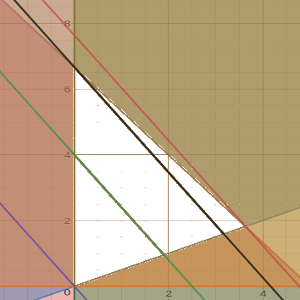
\includegraphics[width=0.8\textwidth]{q5b.png}
\caption{ Feasible Set and Level Sets }
\end{figure}

The feasible set is the white section that forms the intersectio of all the partitions described by the constraints. It is clear from the graph that the optimal solution is obtained at at the furthest right intersection, located at: $( \frac{40}{11},\frac{20}{11})$ and has value: $\frac{2500}{11}$ 

\subsection*{Part c.}
The binding contraints are the lines that the optimal solution is on, namely: $x - 2y \leq 0$ and $4x + 3y \leq 20$ 
\newline
The nonbinding constraints are the remaining constraints: $x \geq 0$ and $y \geq 0$.

\subsection*{Part d.}
The first constraint changes to: $4x+3y\leq 30$ 

\begin{figure}[!h]
\centering
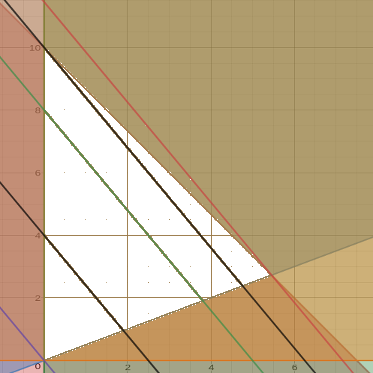
\includegraphics[width=0.8\textwidth]{q5d.png}
\caption{ Feasible Set and Level Sets }
\end{figure}

The new feasible set is the white section, and the optimum will occur where the red line intersects the feasible set. This point is: $(\frac{60}{11}, \frac{30}{11})$ and the new maximum is: $\frac{3150}{11}$

\end{document}
